\subsection{INEPT and product operators}
\label{subsec:theory__inept}

\begin{figure}[htbp]
    \centering
    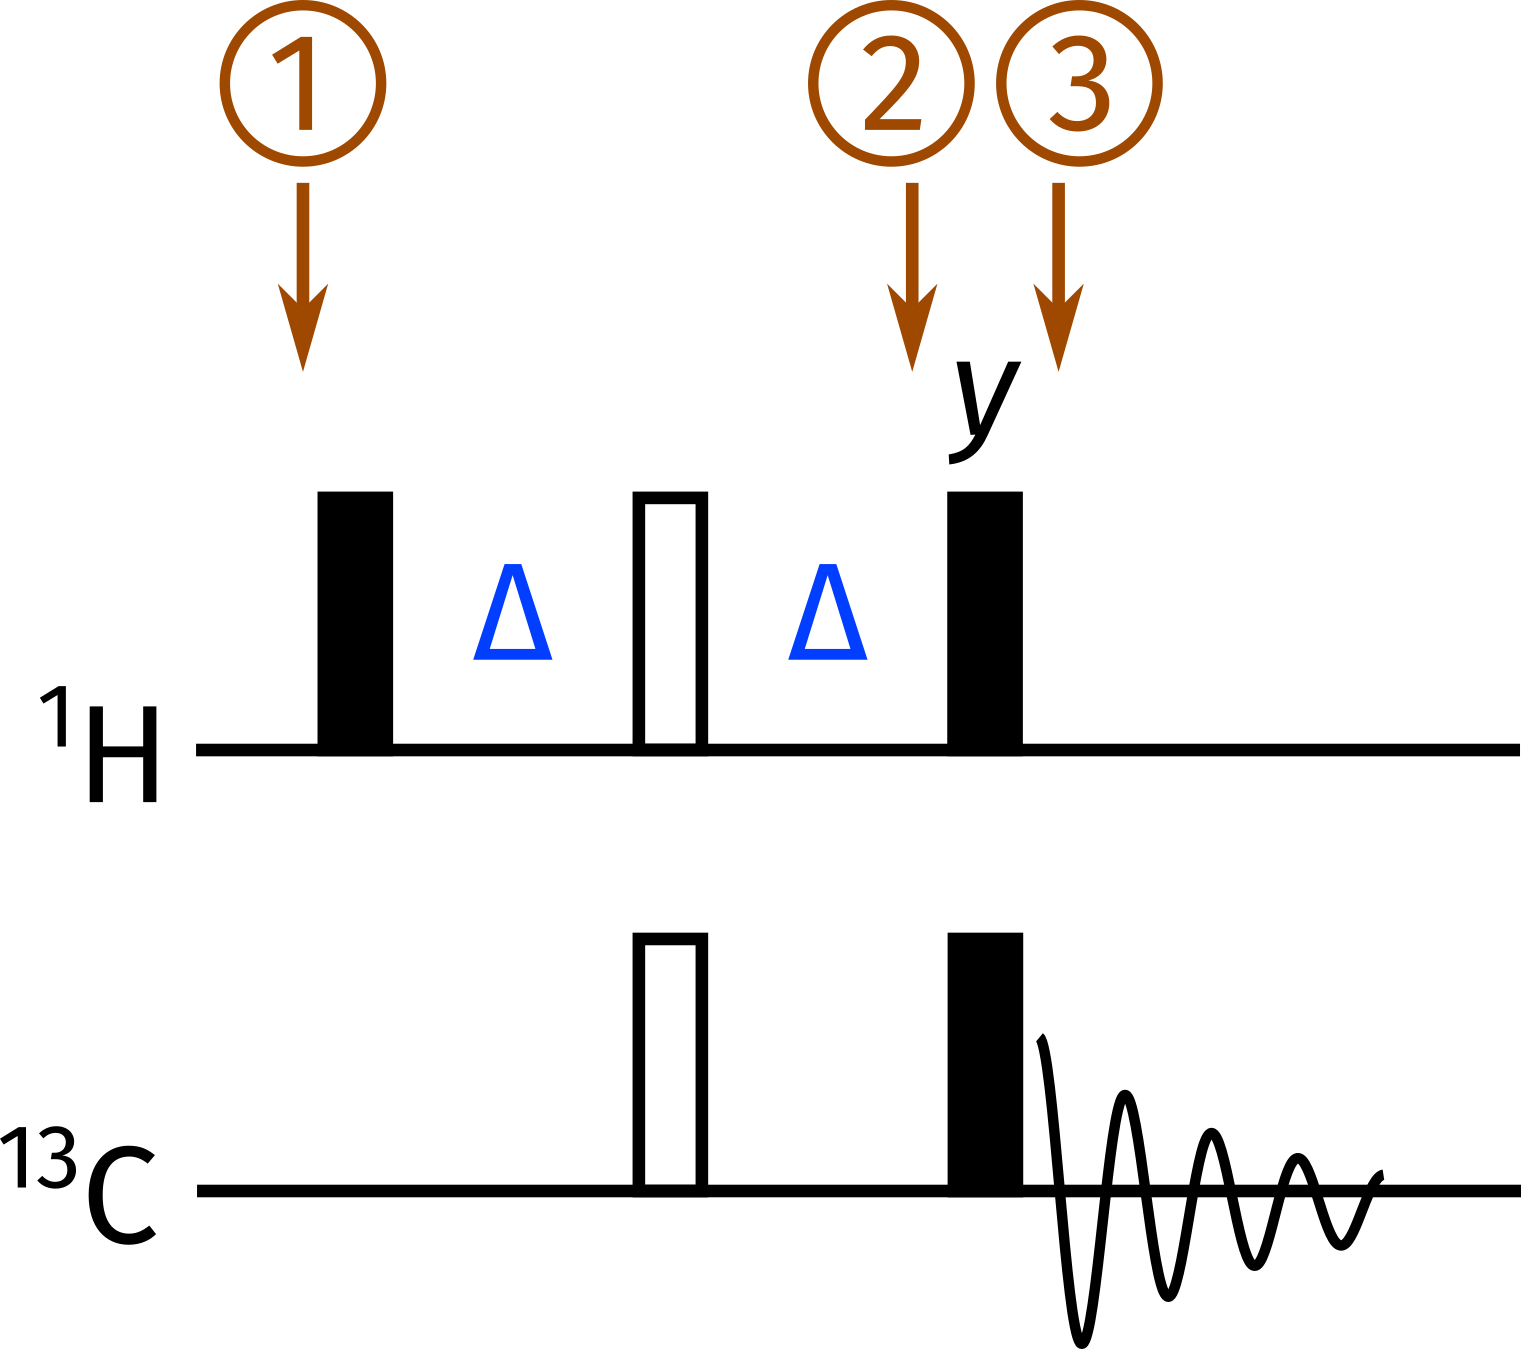
\includegraphics[]{pp/inept.png}%
    \caption[INEPT pulse sequence]{
        INEPT pulse sequence.
        The delay $\Delta$ is set to $1/(4 \cdot \oneJ{CH})$.
    }
    \label{fig:inept}
\end{figure}

Having tackled a simple single-spin case, we now move to the analysis of coupled spin systems and the development of the so-called `product operator formalism'.\autocite{Sorensen1984PNMRS}
In particular, we look at the INEPT experiment\autocite{Morris1979JACS,Morris1980JACS}, in which magnetisation is transferred from a nuclide with a high magnetogyric ratio to one with a low magnetogyric ratio through a scalar coupling: for example, from \proton{} to \carbon{} using the one-bond coupling constant, $\oneJ{CH}$ (\cref{fig:inept}).
Following tradition, the two nuclei are respectively labelled $I\/$ and $S$.%
\footnote{This may seem insensible since $I\/$ is the \textit{sensitive} and $S$ the \textit{insensitive} nucleus, and indeed, in the original INEPT literature\autocite{Morris1979JACS} the meanings of $I\/$ and $S$ were swapped. However, this usage has not been universal\autocite{Pines1972JCP}, and in modern usage the identification of $I\/$ as the sensitive nucleus seems to have prevailed.}
The Schr\"odinger-picture free Hamiltonian for a weakly coupled system (cf.\ \cref{eq:weak_coupling,eq:h_j_secular}) is $\Hfree = \omega_{0,I} I_z + \omega_{0,S} S_z + 2\cpi J_{IS} I_z S_z$.
At the very beginning of the sequence (point \circled{1}), we formally have the equilibrium density operator
\begin{equation}
    \label{eq:density_eqm_heteronuclear_full}
    \rho_0 = \frac{\exp(-\beta\hbar\Hfree)}{\Tr[\exp(-\beta\hbar\Hfree)]}
    \approx E - \beta\hbar (\omega_{0,I} I_z + \omega_{0,S} S_z + 2\cpi J_{IS} I_z S_z),
\end{equation}
using the same approximations as in \cref{eq:nmr_equilibrium_rho}.
The scalar coupling term can be safely neglected as $2\cpi J_{IS}$ is several orders of magnitude smaller than the Larmor frequencies $\omega_0$.
After removing the physically irrelevant $E\/$ term and factoring out a constant of $\beta\hbar B_0$, we end up with:
\begin{equation}
    \label{eq:density_eqm_heteronuclear_simplified}
    \rho'_0 = \gamma_I I_z + \gamma_S S_z.
\end{equation}
This represents equilibrium magnetisation (or \textit{polarisation}) on both spins $I\/$ and $S$, in proportion to their magnetogyric ratios.
In general, an NMR experiment may manipulate---and ultimately detect---both of these terms.
Since unitary evolution according to the Liouville--von Neumann equation is \textit{linear}, in that $U(\rho_1 + \rho_2)\adj{U} = U\rho_1\adj{U} + U\rho_2\adj{U}$, we can treat these two terms separately: we focus first on the spin-$I\/$ polarisation, $\rho_I = \gamma_I I_z$.
The first \angang{90}{x} \proton{} pulse tips this magnetisation into the transverse plane (ignoring off-resonance effects):
\begin{equation}
    \label{eq:rho_after_pulse_x}
    \rho_I \to \exp[-\mi(\cpi/2) I_x] \gamma_I I_z \exp[\mi(\cpi/2) I_x] = -\gamma_I I_y.
\end{equation}
In principle, we could continue in this manner through repeated application of the `sandwich' formulae (\cref{eq:sandwich_formula_1,eq:sandwich_formula_2}, as well as an analogous version for the $I_zS_z$ term). 
For example, in the $\Delta$ delay which follows, we have that
\begin{equation}
    \label{eq:rho_after_delay_x}
    \begin{aligned}
        \rho_I &\to -\gamma_I\exp(-\mi\HfreeI\Delta) I_y \exp(\mi\HfreeI\Delta) \\
               &= -\gamma_I\exp(-\mi\HJ\Delta)\exp(-\mi\Hoffset\Delta) I_y \exp(\mi\Hoffset\Delta)\exp(\mi\HJ\Delta) \\
               &= \ldots
    \end{aligned}
\end{equation}
When performing simulations of NMR experiments, such as those in later chapters, this is precisely what happens, with the slight difference that the Liouville--von Neumann equation (\cref{eq:lvn_interaction_integrated}) is evaluated numerically rather than symbolically.
Note that in going from the first to the second line, we can only `split up' $\HfreeI$ into its constituent components $\Hoffset$ and $\HJ$ because they commute.

\begin{figure}[htbp]
    \centering
    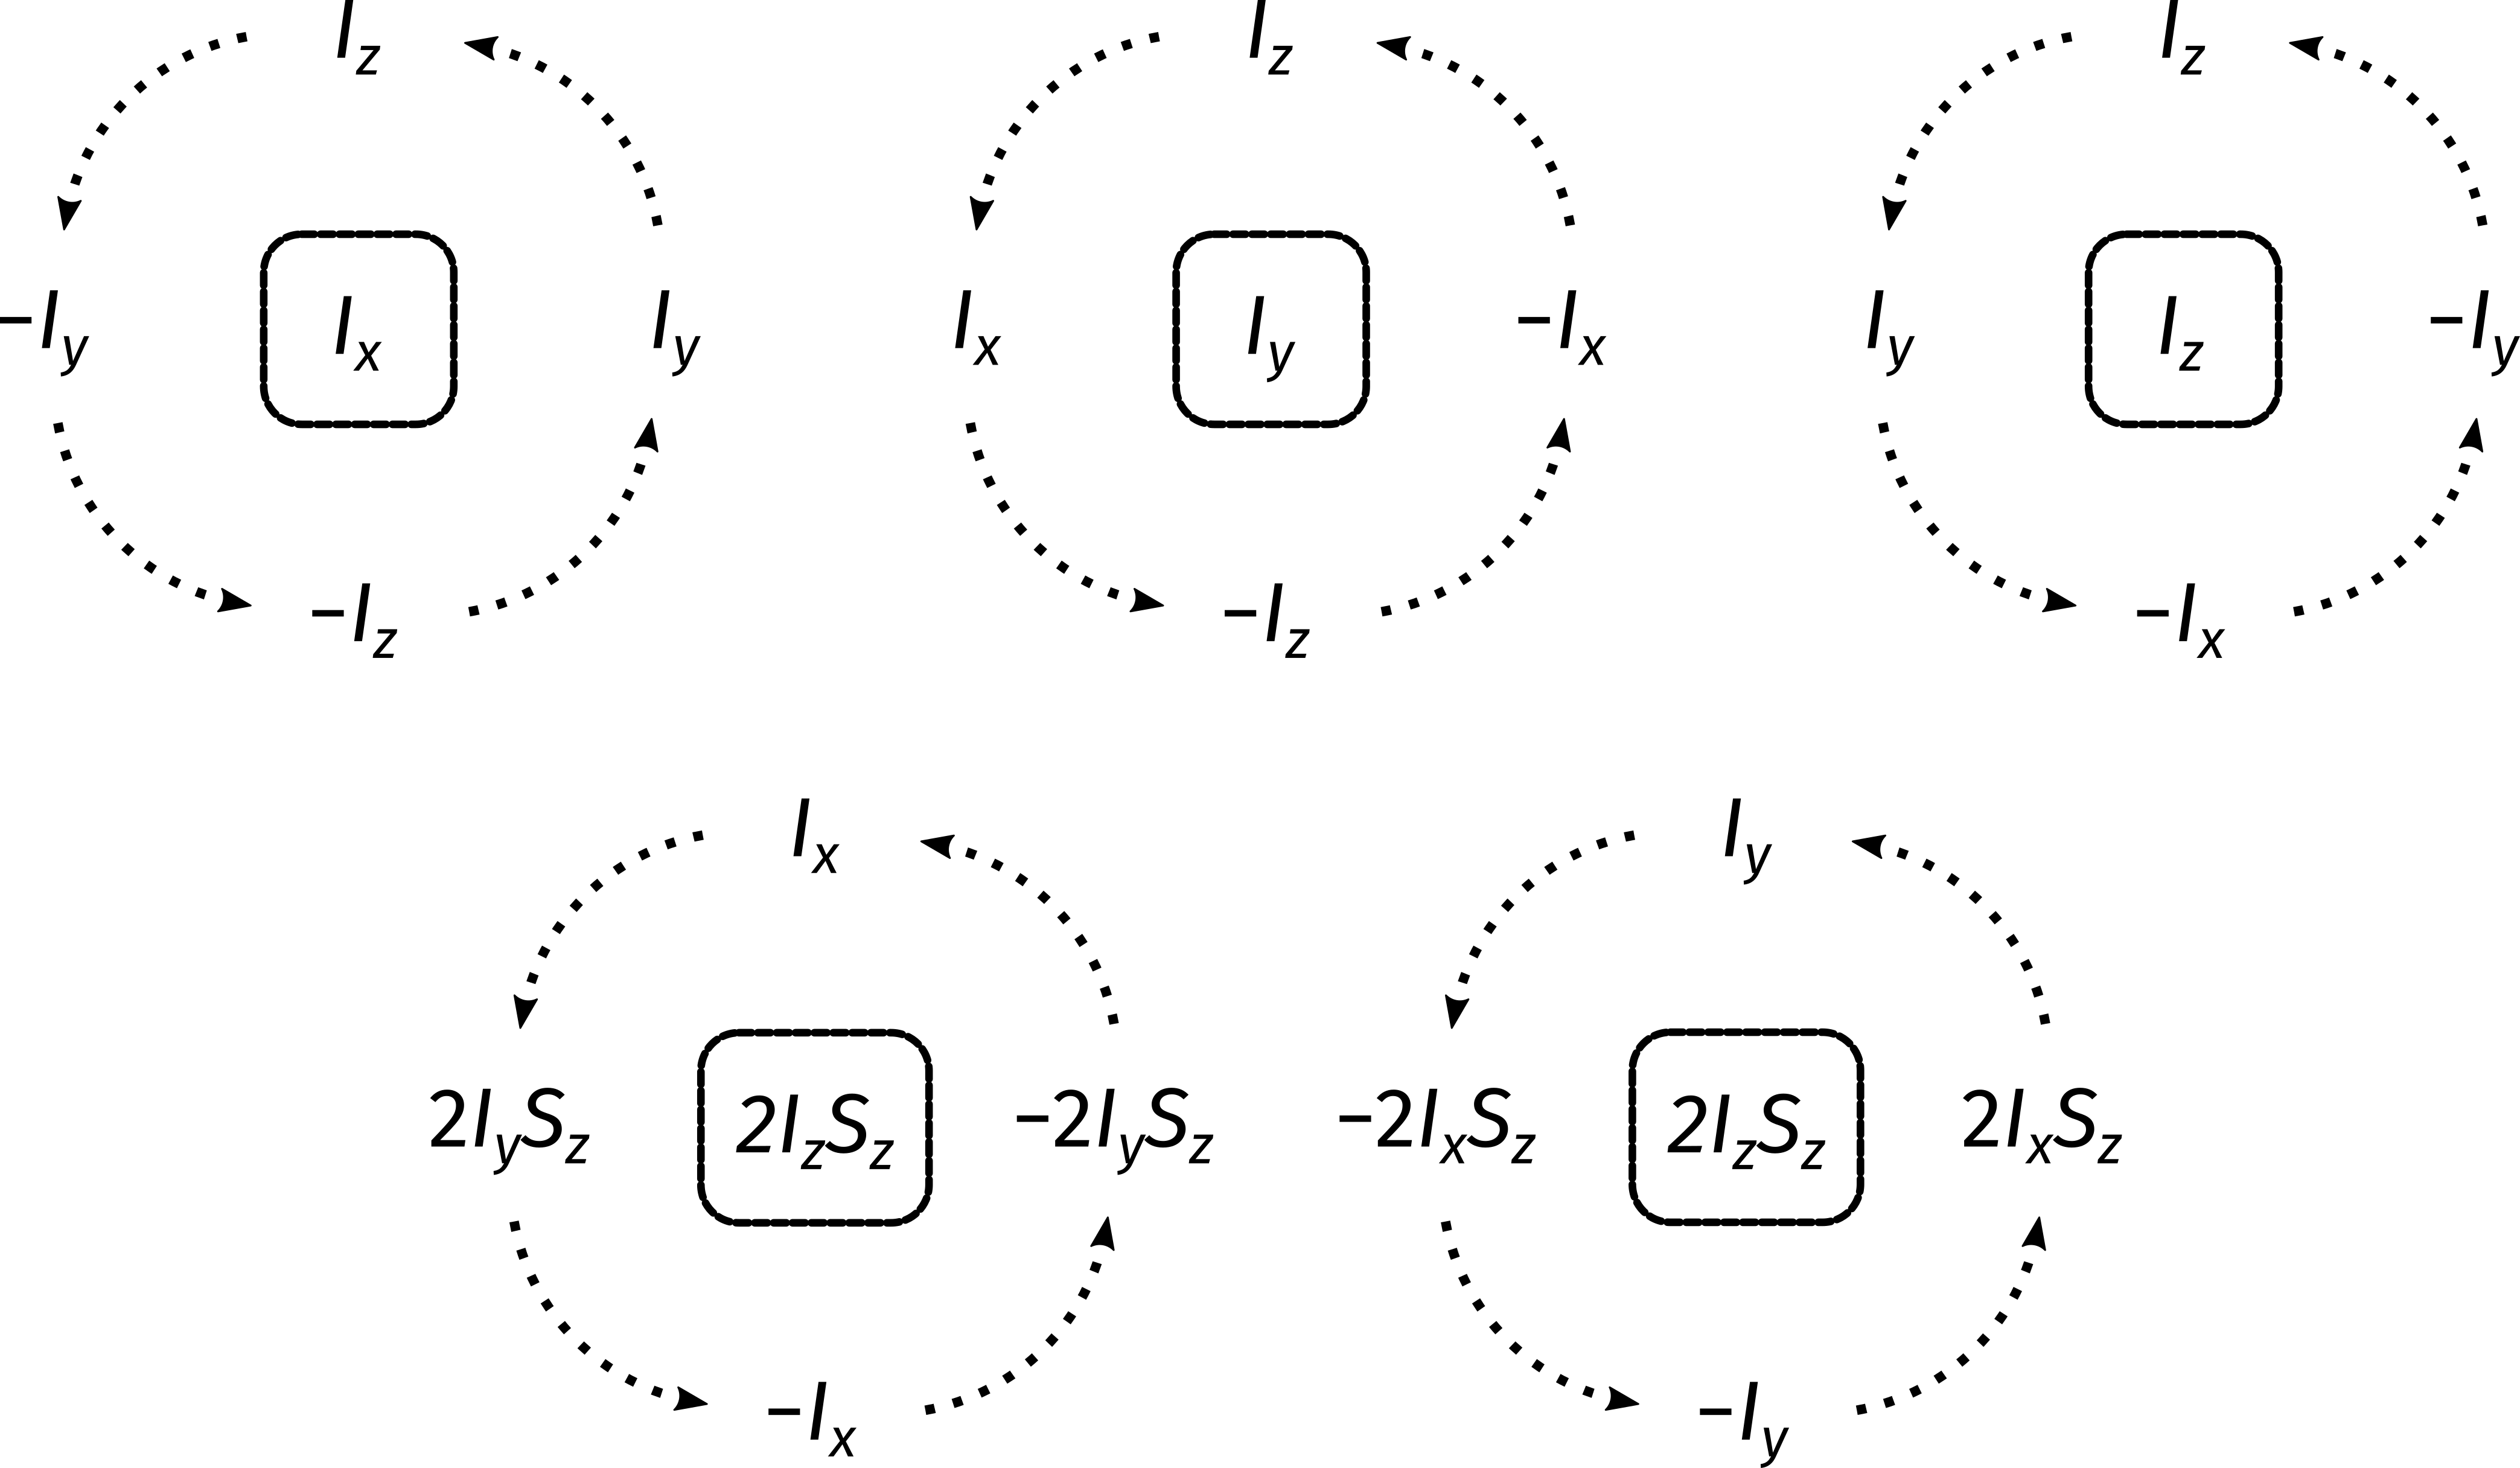
\includegraphics[]{theory/prodop_rules.png}%
    \caption[Simplified rules for product operator evolutions]{
        Simplified rules for the evolution of product operators under different common Hamiltonians (offset, weak/secular J-coupling, and pulses).
        These Hamiltonians often have the form $\omega M$ where $M$ is some `base operator', and are applied for a time $\tau$.
        The boxed operators in the centre of each group refer to $M$; the initial state is then `rotated' about this by an angle of $\omega\tau$ to obtain the final state, or more formally, it is transformed into itself times $\cos(\omega\tau)$, plus the next term in the cycle times $\sin(\omega\tau)$.
        For example, a \angang{90}{x} pulse has the `base' operator $I_x$ and the angle $\omega\tau = \cpi/2$; thus, the initial state $I_z$ would be rotated to $I_z\cos(\cpi/2) - I_y\sin(\cpi/2) = -I_y$.
    }
    \label{fig:prodop_rules}
\end{figure}

When analysing pulse sequences by hand, however, it is far more convenient to use a set of heuristics which summarise the effects of various pulse sequence elements.
For example, \cref{fig:prodop_rules} summarises the evolution of a density operator under a single term of the Hamiltonian: as above, since $[\Hoffset, \HJ] = 0$, we only need to consider one term at a time.
More high-level rules may be devised as well: for example, during the $\Delta$--\angang{180}{x}$(I,S)$--$\Delta$ spin echo which comes next, the $J_{IS}$ interaction in $\HfreeI$ is allowed to evolve for a period of $2\Delta$, but the offset term is \textit{refocused} and can be ignored.
(The sign inversion caused by the \ang{180} pulses must also be included.)
As per \cref{fig:prodop_rules}, this transforms the $-I_y$ term to $-2I_xS_z$ at point \circled{2}: the Hamiltonian is $\cpi J_{IS} 2I_zS_z$ for a total time of $2\Delta = 1/(2J_{IS})$, so the `angle' rotated through is $\cpi J_{IS}/(2J_{IS}) = \cpi/2$.
Immediately after this, the \angang{90}{x}$(I,S)$ pair of pulses rotates this magnetisation to $-2I_zS_y$ (point \circled{3}).
These transformations are often denoted with simpler notation:
\begin{equation}
    \label{eq:inept_prodop}
    \gamma_I I_z
    \xrightarrow{\angang{90}{x}(I)} -\gamma_I I_y
    \xrightarrow{\Delta\text{--}\angang{180}{x}(I,S)\text{--}\Delta} -2\gamma_I I_xS_z
    \xrightarrow{\angang{90}{y}(I),\angang{90}{x}(S)} -2\gamma_I I_zS_y
\end{equation}
During the detection period, the term $-2\gamma_II_zS_y$ evolves as
\begin{align}
    \label{eq:inept_fid_prodop}
    -2\gamma_I I_zS_y \xrightarrow{\HfreeI} -2\gamma_I I_zS_y\cos(\Omega_St)\cos(\cpi Jt) + \gamma_I S_x\cos(\Omega_St)\sin(\cpi Jt) \notag{} \\
    \qquad {} - 2\gamma_I I_zS_x\sin(\Omega_St)\cos(\cpi Jt) + \gamma_I S_y\sin(\Omega_S t)\sin(\cpi Jt),
\end{align}
from which we extract the complex signal
\begin{equation}
    \label{eq:inept_fid}
    s_I(t) = \langle S_x(t) \rangle + \mi \langle S_y(t) \rangle = \frac{\gamma_I}{2\mi}\bigl\{\exp[\mi(\Omega_S + \cpi J_{IS})t] - \exp[\mi(\Omega_S - \cpi J_{IS})t]\bigr\}.
\end{equation}
After Fourier transformation, the resulting spectrum has two peaks with opposite phase and have the frequencies $\Omega_S \pm \cpi J_{IS}$; because of the factor of $1/(2\mi)$, the real part of the spectrum will contain dispersion-mode signals (\cref{fig:doublet_lorentzians_dis_anti}).
If desired, zeroth-order phase correction can be performed here, yielding instead a pair of absorption-mode signals still with opposite phases (\cref{fig:doublet_lorentzians_abs_anti}).
In either case, this is termed an \textit{antiphase} doublet; the product operators which give rise to it ($2I_zS_x$ and $2I_zS_y$) are said to be antiphase with respect to spin $I\/$.
Importantly, the amplitude of the signal scales as $\gamma_I$ rather than $\gamma_S$; since $\gamma_I > \gamma_S$, this represents a sensitivity enhancement compared to the direct excitation of $S$-magnetisation.

\begin{figure}[htbp]
    \centering
    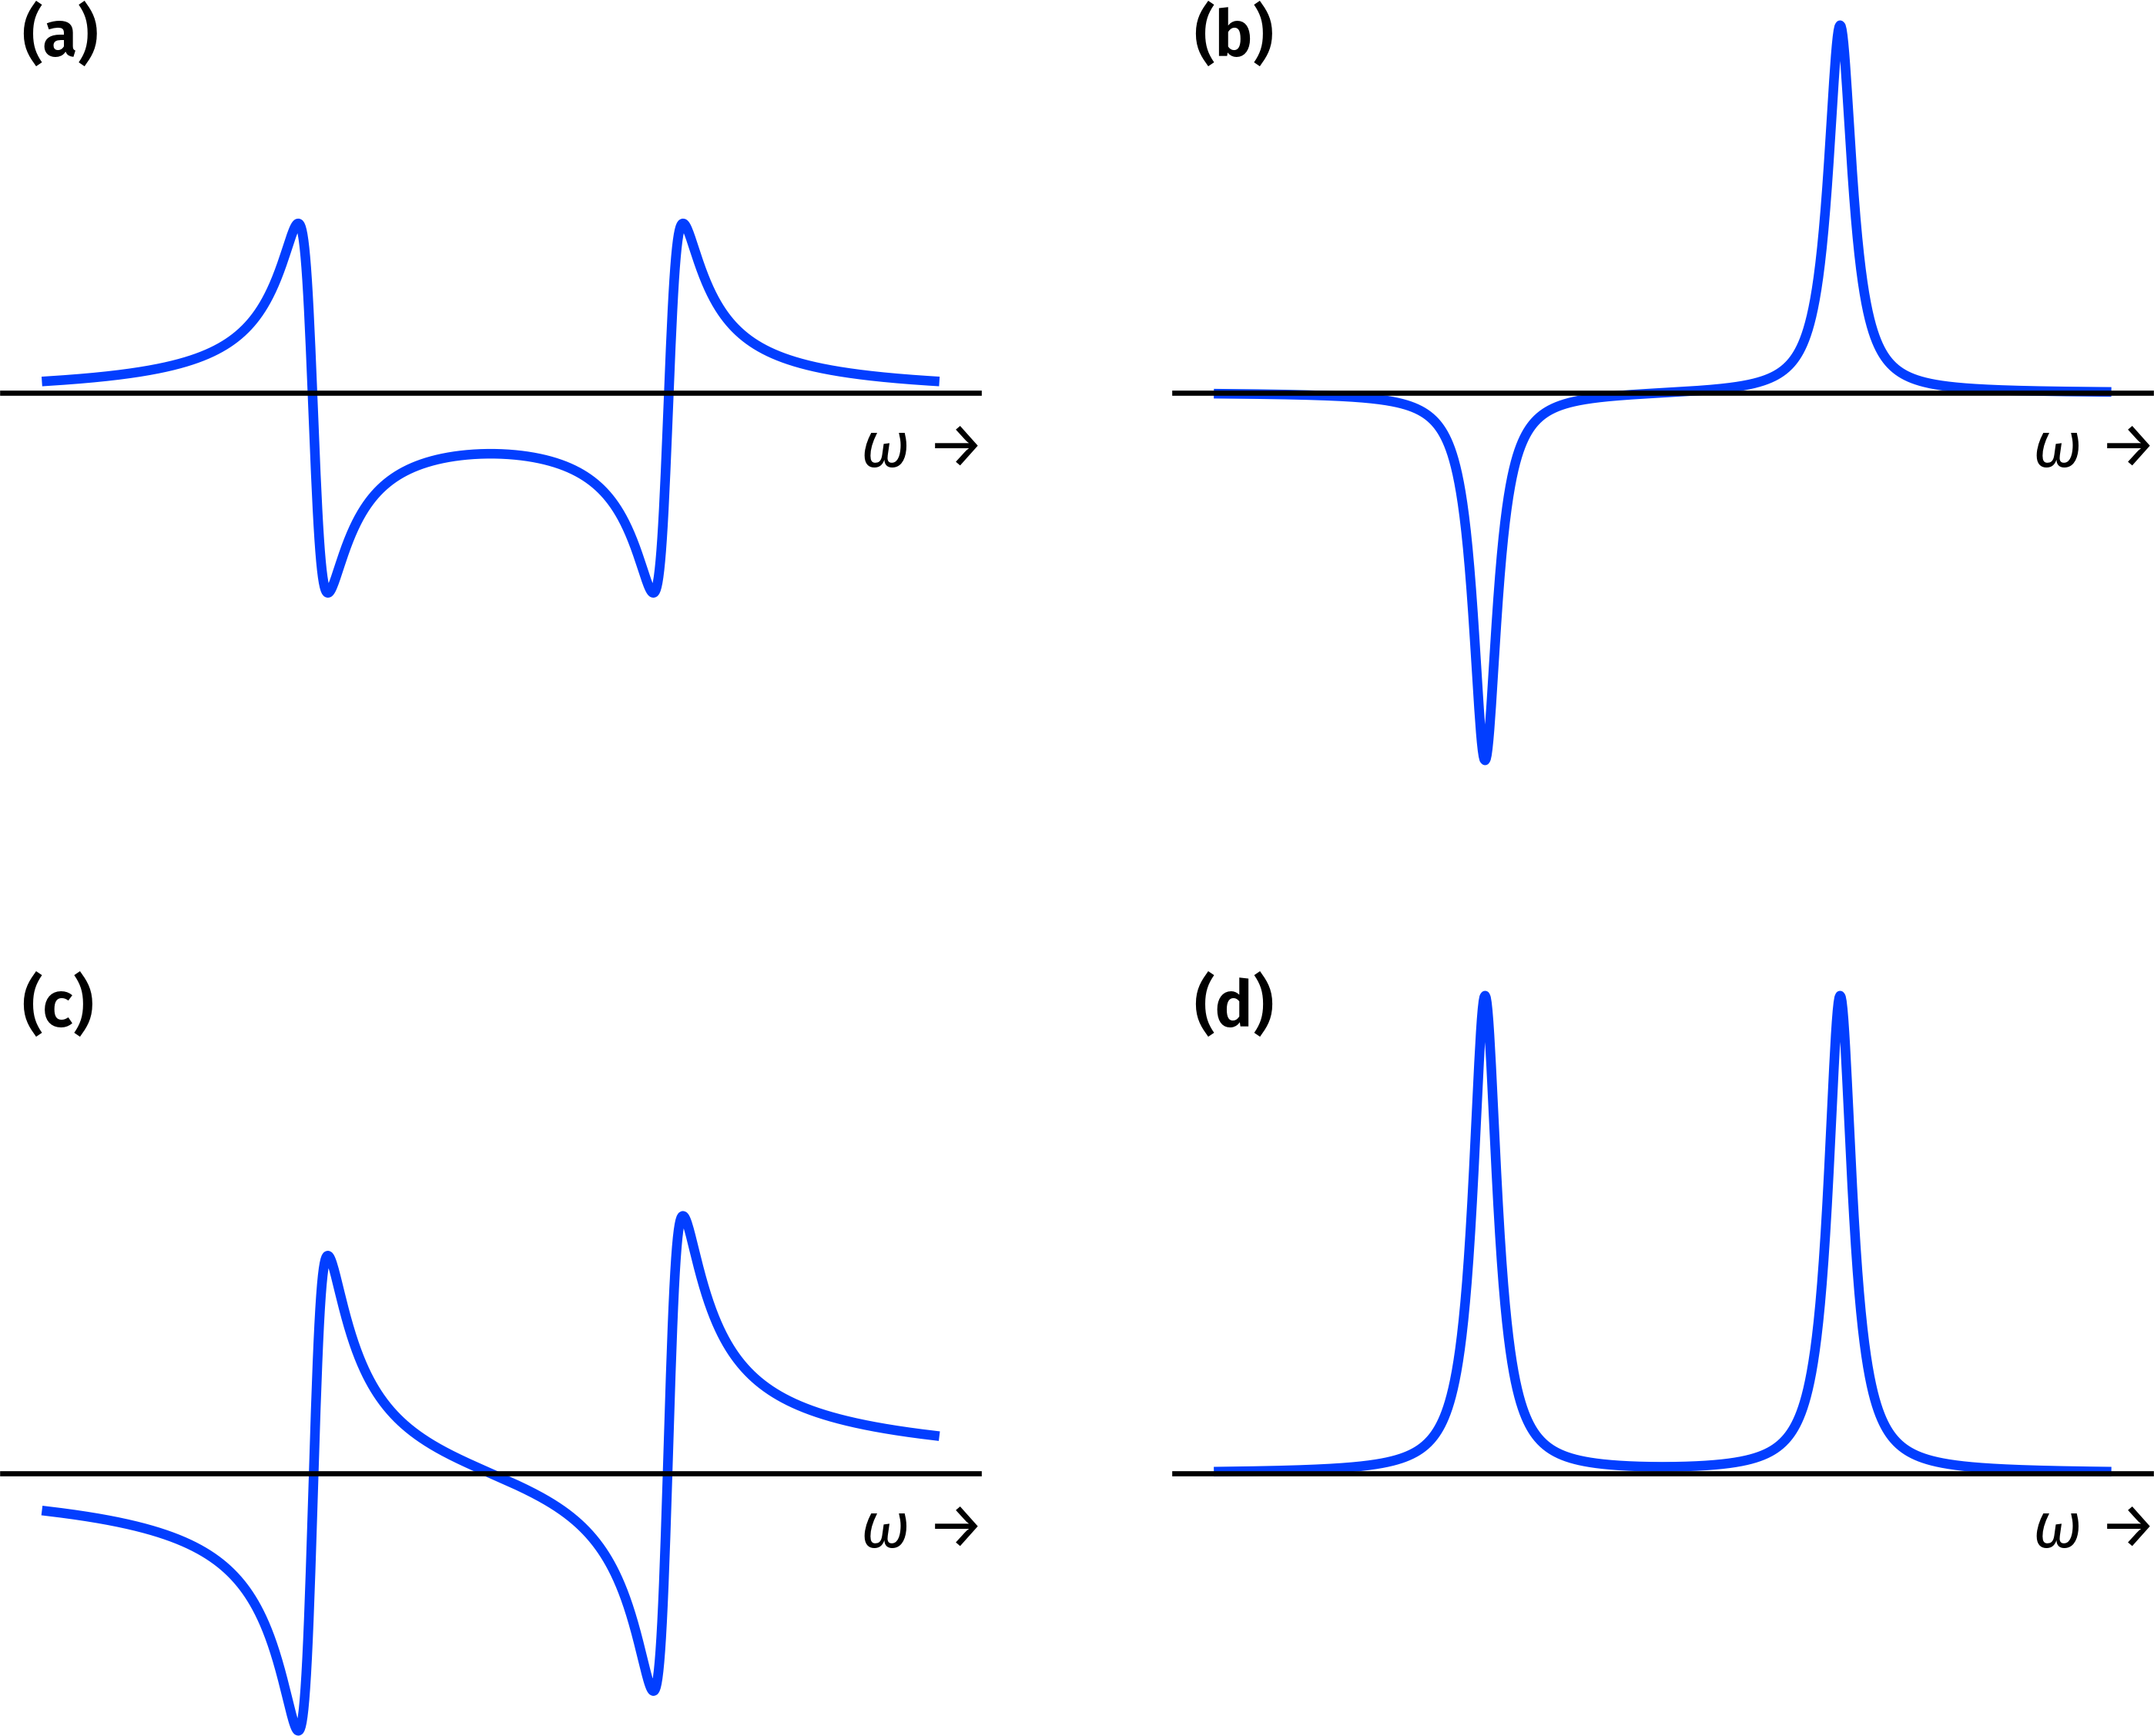
\includegraphics[]{theory/doublet_lorentzians.png}%
    {\phantomsubcaption\label{fig:doublet_lorentzians_dis_anti}}%
    {\phantomsubcaption\label{fig:doublet_lorentzians_abs_anti}}%
    {\phantomsubcaption\label{fig:doublet_lorentzians_dis_in}}%
    {\phantomsubcaption\label{fig:doublet_lorentzians_abs_in}}%
    \caption[Absorption- and dispersion-mode in-phase and antiphase doublets]{
        Peak shapes of a doublet.
        In all cases, the separation between the two peaks is $2\cpi J_{IS}$.
        \textbf{(\subref*{fig:doublet_lorentzians_dis_anti})} Antiphase, dispersion-mode.
        \textbf{(\subref*{fig:doublet_lorentzians_abs_anti})} Antiphase, absorption-mode.
        \textbf{(\subref*{fig:doublet_lorentzians_dis_in})} In-phase, dispersion-mode.
        \textbf{(\subref*{fig:doublet_lorentzians_abs_in})} In-phase, absorption-mode.
    }
    \label{fig:doublet_lorentzians}
\end{figure}

Of course, this is only half of the picture; we have not considered what happens to the other part of the magnetisation, namely $\rho_S = \gamma_S S_z$.
Clearly, this is unaffected by the initial $\angang{90}{x}(I)$ pulse and the first $\Delta$ delay.
The $\angang{180}{x}(S)$ pulse inverts it, and the final $\angang{90}{x}(S)$ pulse in fact transforms it into observable $S$-magnetisation:
\begin{equation}
    \label{eq:inept_prodop_s}
    \gamma_S S_z \xrightarrow{\angang{90}{x}(I)\text{--}\Delta} \gamma_S S_z
    \xrightarrow{\angang{180}{x}(I),\angang{180}{x}(S)\text{--}\Delta} -\gamma_S S_z
    \xrightarrow{\angang{90}{y}(I),\angang{90}{x}(S)} \gamma_S S_y
\end{equation}
This term produces \textit{in-phase} spin-$S$ magnetisation during the detection period (where the two components of the doublet have the same phase):
\begin{equation}
    \label{eq:inept_fid_S}
    s_S(t) = \frac{\mi\gamma_S}{2}\bigl\{\exp[\mi(\Omega_S + \cpi J_{IS})t] + \exp[\mi(\Omega_S - \cpi J_{IS})t]\bigr\},
\end{equation}
Because of the factor of $\mi$, the real part of the spectrum will contain a dispersion-mode doublet (\cref{fig:doublet_lorentzians_dis_in}).
The signal actually measured by the spectrometer is $s(t) = s_I(t) + s_S(t)$; and the spectrum is a weighted sum of in-phase and antiphase magnetisation.
This leads to potentially unwanted phase distortions in the spectrum, which one would prefer to suppress.

This can be accomplished through the technique of \textit{phase cycling}, where pulse and receiver phases are changed in concert and the resulting FIDs summed in order to select for a particular signal.
In this case, the INEPT experiment is performed twice, once with the phases as given in \cref{fig:inept}, and once where the initial $\angang{90}{x}(I)$ pulse is replaced with a $\angang{90}{-x}(I)$ pulse.
The first of these gives us the same signals as above.
However, inverting the initial $I\/$ pulse leads to $s_I$ acquiring a minus sign, because the initial $I_z$ term is rotated to $I_y$ instead of $-I_y$.
On the other hand, the signal component $s_S$ is unaffected by this pulse and thus does not experience a change of sign.
The two FIDs we record are thus as follows:
\begin{align}
    \label{eq:inept_phase_cycling}
    s_1(t) &= s_I(t) + s_S(t) \\
    s_2(t) &= -s_I(t) + s_S(t)
\end{align}
Simply taking the difference of these two FIDs yields a signal where the desired $s_I$ has been accumulated and $s_S$ has been cancelled out.
In practice, instead of subtracting the two signals, it is typical to shift the receiver phase $\phirec$ by \ang{180} in the second experiment: this introduces a phase shift of $\exp(-\mi\cpi) = -1$ to the signal, and the two signals can now be \textit{added} together instead of subtracted to cancel out $s_S$.
Since both $\phi_1$ and $\phirec$ are $0$ on the first experiment and $\cpi$ on the second experiment, we can express this as $\phi_x = \phirec = (0, \cpi)$.
This is more commonly denoted as $\phi_1 = \phirec = (x, -x)$, because the phases $(0, \cpi)$ correspond to the $+x$- and $-x$-axes respectively.

The `simplified' analysis of pulse sequences shown in \cref{eq:inept_prodop,eq:inept_prodop_s} is often called \textit{`product operator'} analysis\autocite{Sorensen1984PNMRS}, because the underlying two-spin operators are products of single-spin Cartesian operators.
Although this is often touted as being `simpler' than full density operator calculations, it is really just a shorthand which masks the quantum mechanical theory developed in this chapter:
\begin{equation}
    \label{eq:product_operator_shorthand}
    \underbrace{I_z \xrightarrow{\angang{90}{x}(I)} -I_y}_{\textit{product operator}}
    \quad\Longleftrightarrow\quad
    \underbrace{\exp(-\mi I_x\cpi/2)I_z\exp(\mi I_x\cpi/2) = -I_y}_{\textit{density operator}}
\end{equation}
Since the operators $\{E, I_x, I_y, I_z\}$ form a complete basis for a single-spin system, their products (i.e.\ product operators) likewise form a complete basis for multiple-spin systems, and so \textit{any} density matrix for a multiple-spin system may be expressed as a linear combination of product operators.
Thus, strictly speaking, the use of product operators therefore does not actually sacrifice any power in and of itself.
However, the heuristics such as those in \cref{fig:prodop_rules} \textit{are} limiting, in that the evolution under some Hamiltonians---for example, strong coupling $\symbf{I}\cdot\symbf{S}$, or pulses for off-resonance spins where $H\/$ is a sum of $I_x$ and $I_z$---cannot be neatly captured in such a pictorial form.
